\chapter{Background}
\label{chapter:Background}

This chapter provides an overview of the relevant background information used in completing this thesis. This chapter centres around the chosen greenhouse model and the rationale behind its selection. It delves into the principles of RL and MPC, and finally provides information on the necessity of combining these algorithms. 

\section{Greenhouse Model}
\label{section:greenhouse-model}

The accuracy and complexity of the model at hand directly impacts the quality of the control.  The dynamics of a greenhouse can be characterized through various modeling approaches depending on its application. Methods such as Computational FLuid Dynamics (CFD) are used to develop numerical models of the indoor climate of a greenhouse using partial differentiable equations. In recent years, CFD simulations have become increasingly more accurate in simulating indoor greenhouse climate \cite{delatorre-geaComputationalFluidDynamics2011}, however extensive knowledge and computational power of the system is required.
Their complexity makes them intractable for mathematical solvers such as MPC and they present substantial challenges for learning in model-free methods, resulting in a demanding and laborious training process \cite{jansenOptimalControlLettuce2023}.Simplified models of greenhouse dynamics are developed by assuming homogeneity in the greenhouse climate and neglecting the impact of wall effects. Additional assumptions about $CO_2$ and humidity are incorporated to yield a model conducive to  control applications, as discussed in \cite{jansenOptimalControlLettuce2023, lopez-cruzDevelopmentAnalysisDynamical2018}. While these simplified models sacrifice some accuracy in representing the system, they significantly reduce computational demands, thereby making them tractable for mathematical solvers. These mechanistic process models are often derived from first principles and use ordinary differential of difference equations to represent the system dynamics.
In contrast, Data-drive models such as in \cite{gongDeepLearningBased2021} and \cite{maestriniMixingProcessbasedDatadriven2022} have also been used to create a black box model of the greenhouse dynamics. Although such models may yield accurate results, they do so only in the environment wherein the data originates from, whereas mechanistic process models often generalize better to different environments and situations. Although such black box models may be used for RL, they could pose challenges for mathematical solvers due to their potential complexity and/or unknown mathematical makeup.
Similar models and scenarios exist for crops. In some cases, it is possible to model crops with a single variable (namely the crop dry weight) given the climate conditions for simple crops, such as lettuce \cite{royPAPrecisionAgriculture2002}. However, for more complicated crops such as tomatoes and cucumber additional  information is required to describe their growth behaviour and life cycle stages \cite{kuijpersModelSelectionCommon2019}. 
\\
Although accurate models may seem appealing, they are often exhibit complexity and entail a high-dimensional state-space. Both factors have adverse effects on model-free RL algorithms and MPC, making such models impractical for the development of optimal control policies. This arises from the fact that, in the case of MPC, finding a tractable solution within the given time constraints may prove challenging. Consequently, it might fail to meet timing requirements and constraints, or even find no solution at all. Similarly, in the context of model-free RL algorithms, the use of highly accurate models could destabilize the learning procedure, making it a more difficult and time-consuming task to learn a policy \cite{lawrynczukMPCAlgorithms2014,dulac-arnoldChallengesRealWorldReinforcement2019}. Therefore, for optimal control, is it desirable to use a low-dimensional simplified model whereby the most important dynamics of the system is still captured. Moreover, the control law obtained from the simplified model may be adjusted and applied to the more accurate models in order to validate them. If however, the control law is not satisfactory, the simplified model must be adapted and a new control policy obtained. Often this leads to an iterative cycle of updating the model and validating the obtained control policy until a satisfactory performance on the high-accurate model is obtained \cite{knibbeDigitalTwinsGreen2022}. Since the thesis focuses on the impact and implementation of merging RL and MPC for optimal control, it is outside of the scope to design and develop a model.
Therefore a validated simplified mechanistic model of a greenhouse with lettuce crops will be selected. Although data driven models may mimic a simplified mechanistic process, a mechanistic process is required for a model predictive controller. 
Due to the relative simplicity of lettuce crop models, they find utility alongside a greenhouse model that assumes an indoor homogeneous climate. A model, which encapsulates the fundamental dynamics of the greenhouse and crops, is detailed in \cite{hentenGreenhouseClimateManagement1994} and has been explicitly developed for optimal control applications. More importantly, the model proposed in \cite{hentenGreenhouseClimateManagement1994} has been validated in \cite{vanhentenValidationDynamicLettuce1994}, and has been extensively utilised in obtaining optimal control policies such as in \cite{jansenOptimalControlLettuce2023,vanstratenOptimalGreenhouseCultivation2010,ghoumariNonlinearConstrainedMPC2005,lubbersAutonomousGreenhouseClimate2023, morcegoReinforcementLearningModel2023}. Therefore, the choice was made to utilise the model suggested in \cite{hentenGreenhouseClimateManagement1994} for this thesis.



\subsection{Model Description}
\begin{figure}[H]
	\centering
	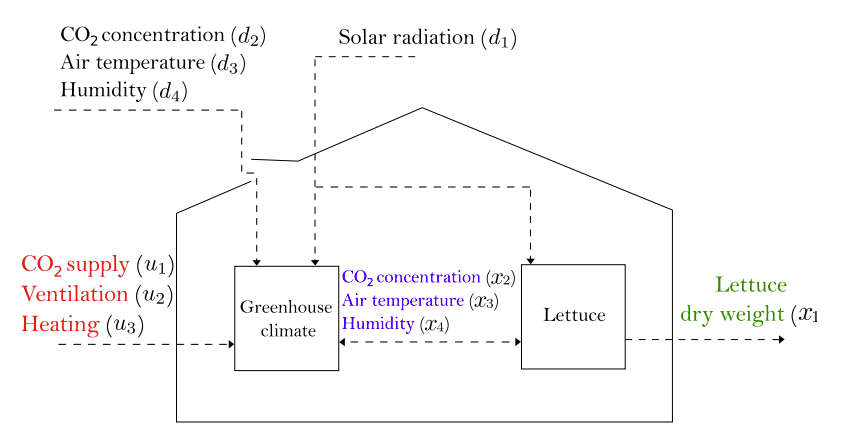
\includegraphics[width = 0.75\linewidth]{figures/van_henten_model.png}
	\caption{Graphical representation of the greenhouse crop production process \cite{hentenGreenhouseClimateManagement1994}}
	\label{fig:van_henten_model}
\end{figure}

\autoref{fig:van_henten_model} displays a graphical representation of the used greenhouse model from the works of \cite{hentenGreenhouseClimateManagement1994}. The control inputs are highlighted in red, the states of the indoor climate in blue, the state of the crops in green and the external disturbances given in black. The states of the system, control inputs, disturbances and outputs are described in \autoref{eq: model vectors}.

\begin{equation}
	\begin{aligned}
		& x(k) = \begin{bmatrix}
			x_d & x_{C0_2} & x_T & x_h
		\end{bmatrix}^T
		\\
		& u(k) = \begin{bmatrix}
			u_{C0_2} & u_{v} & u_q
		\end{bmatrix}^T
		\\
		& d(k) = \begin{bmatrix}
			d_{Io} & d_{C02} & d_T& d_h
		\end{bmatrix}^T
		\\
		& y(k) = \begin{bmatrix}
			y_d & y_{C0_2} & y_T & y_RH
		\end{bmatrix}^T
	\end{aligned}
	\label{eq: model vectors}
\end{equation}
The state of the system includes Crop dry mass, $C0_2$ density within the greenhouse, the temperature inside the greenhouse and the absolute humidity within the greenhouse. Crop dry mass is used since it is a more reliable and accurate measure of the biomass of the plant. Unlike fresh weight, which varies with the plant's water content which is in turn influenced by weather conditions, crop dry mass provides a more stable and consistent metric. The control vector encapsulates the $C0_2$ injection rate, ventilation rate and the heating supply. Furthermore, the disturbances from the weather include the incoming solar radiation, ambient $C0_2$ density, ambient temperature and the ambient humidity content. The measured output is largely the same as the state of the system however the units of the indoor $C0_2$ density and relative humidity differ in that they report in units as used in standard measurement sensors.



\subsection {Model State Equations}

\paragraph{State Equations}
The model described in \cite{hentenGreenhouseClimateManagement1994} is fully described by the crop dry weight, temperature, humidity and $C0_2$ levels of the indoor climate. All variables and their units are given in \autoref{tab:model variables and descriptions} and model constants in \autoref{tab:model constants and descriptions}. These states are modeled through a set of ordinary differentiable equations where the change of crop state is represented as

\begin{equation}
	\frac{dX_d}{dt} = c_{\alpha \beta} \phi_{phot,c}(t) - \phi_{resp,d}(t)
\end{equation}

where $c_{\alpha \beta}$ is the crop yield factor, $\phi_{phot,c}$ is the gross carbon dioxide uptake from canopy photosynthesis (also referred to as canopy photosynthesis rate) and $\phi_{resp,d}$ is the maintenance respiration rate of the respired dry matter. 
The greenhouse $C0_2$ density is described through

\begin{equation}
	\frac{dX_{C0_2}}{dt} = \frac{1}{c_{cap,c}}(-\phi_{phot,c}(t) + \phi_{resp,c}(t) + u_{C0_2}(t) \cdot 10^{-6} - \phi_{vent,c}(t))
\end{equation}

where $c_{cap,c}$ is the volumetric $C0_2$ capacity of the greenhouse, $\phi_{resp,c}$ is the respiration rate of $C0_2$ of the crop and $\phi_{vent,c}$ is the  leakage of $C0_2$ through the vents of the greenhouse. Similarly, the change in greenhouse temperature is modeled by the following ODE:

\begin{equation}
	\frac{dX_{Temp}}{dt} = \frac{1}{c_{cap,q}}(u_{q}(t) - Q_{vent,q}(t) + Q_{Io,q}(t))
\end{equation}

where $c_{cap,q}$ is the effective heat capacity of the greenhouse, $Q_{vent,q}(t)$ describes the heat energy exchange between the outside climate and the indoor climate through the greenhouse cover and vents and lastly $Q_{Io,q}(t)$ denotes the heat energy received from the incoming irradiance.

Finally, the humidity of the greenhouse is described by

\begin{equation}
	\frac{dX_{H}}{dt} = \frac{1}{c_{cap,h}}(\phi_{transp,h}(t) - \phi_{vent,h}(t))
\end{equation}
whereby $c_{cap,h}$ is the volumetric humidity capacity of the greenhouse, $\phi_{transp,h}$ models the transpiration rate of the canopy and $\phi_{vent,h}$ is the leakage of water vapour through the vents of the greenhouse.

\paragraph{Process Equations}
The gross canopy photosynthesis rate $\phi_{phot,c}$ is defined as below:
\begin{equation}
	\phi_{phot,c}(t) = (1 - e^{-C_{LAI,d} x_d(t)}) \frac{c_{Io}^{phot} d_{Io}(t) \cdot \phi(t)}{c_{Io}^{phot} d_{Io}(t) +\phi(t)}
	\label{eq: canopy photosynthesis rate}
\end{equation}
where $C_{LAI,d}$ is the effective canopy surface and $c_{Io}^{phot}$ is the light use efficiency. $\phi(t)$ is unit-less as is calculated below as:

\begin{equation}
	\phi (t) = ( -c_{C0_2,1}^{phot} x_T(t)^2 +  c_{C0_2,2}^{phot} x_T(t) - c_{C0_2,3}^{phot} )( x_{C0_2}(t) - c^{phot})
	\label{eq: model phi}
\end{equation}
where $c_{C0_2,1}^{phot},c_{C0_2,2}^{phot},c_{C0_2,3}^{phot}$ indicate the effect of temperature on the gross canopy synthesis rate and $c^{phot}$ is the $C0_2$ compensation point. The maintenance respiration rate of the crop dry matter is described as:

\begin{equation}
	\phi_{resp,d}(t) = c_{resp,d} \cdot \phi_{resp}(t)
	\label{eq:maintenance respiration rate}
\end{equation}

where $c_{resp,d}$ is the respiration rate coefficient of the crop dry matter respiration, $\phi_{resp}(t)$ is the respiration maintenance and can be calculated by:

\begin{equation}
	\phi_{resp}(t) = x_d(t) \cdot c_{Q_{10},resp}^{(x_T(t)-25)/10}
	\label{ respiration maintenance}
\end{equation}
where $ c_{Q_{10},resp}$ indicates the maintenance respiration factor and shows how the respiration maintenance of the crops doubles for every increase of $10^{\circ}C$ and vice versa.
Similarly. the $C0_2$ respiration rate of the crop is calculated by:

\begin{equation}
	\phi_{resp,c}(t) = c_{resp,C0_2} \cdot \phi_{resp}(t)
	\label{ co2 respiration rate}
\end{equation}
where $c_{resp,C0_2}$ is the respiration rate coefficient of $C0_2$ release of the crop. Furthermore, the mass exchange of $C0_2$ is calculated by:

\begin{equation}
	\phi_{vent,c}(t) = (u_v(t) \cdot 10^{-3} + c_{leak})(x_{C0_2}(t) - d_{C0_2}(t))
	\label{eq:co2 exchange}
\end{equation}
where $c_{leak}$ represents the ventilation leakage through the greenhouse cover. Heat energy exchange through the greenhouse cover and vents is described by:

\begin{equation}
	Q_{vent,q}(t) = (c_{cap,v}u_v(t) + c_{go})(x_T(t) - d_T(t))
	\label{heat exchange}
\end{equation}
where $c_{cap,v}$ is the heat capacity per volume of greenhouse air and $c_{go}$ is the heat energy exchange through the greenhouse cover. The heating provided by the irradiance is described by:

\begin{equation}
	Q_{I_o,q}(t) = c_{og}^{rad} d_{I_o}(t)
\end{equation}
Here, $c_{og}^{rad}$ serves as an indicator of the proportion of heating supplied by the irradiance within the greenhouse. Finally. the canopy transpiration rate $\phi_{transp,h}(t)$ and the mass exchange of water vapour through the vents and leaks, $\phi_{vent,h}(t)$ can be expressed:

\begin{equation}
	\phi_{transp,h}(t) = c_{ca}^{evap}(1 - e^{-C_{LAI,d} x_d(t)})\cdot \left( \frac{c_{H_2O,1}^{sat}}{c_R(x_T(t)+c_T)} e^{\frac{c_{H_2O,2}x_T(t)}{x_T(t) + c_{H_2O,3}}} - x_h(t) \right)
\end{equation}

\begin{equation}
	\phi_{vent,h}(t) = (u_v(t) \cdot 10^{-3} + c_{leak})(x_h(t) - d_h(t))
\end{equation}

\paragraph{Output Measurement Equations}
The output measurements for the indoor humidity and $C0_2$ levels are reported in different units via the function $g_{C0_2}(\cdot)$ and $g_h{\cdot}$ respectively.  The output measurements for crop dry mass and indoor temperature correspond to the state variables, as illustrated below:

\begin{equation}
	\begin{aligned}
		& y_d(t) = x_d(t) 
		\\
		& y_{C0_2}(t) = g_{C0_2}(x_T(t),x_{C0_2}(t))
		\\
		& y_T (t) = x_T(t)
		\\
		& y_{RH} = g_h (x_T(t),x_h(t))
	\end{aligned}
\end{equation}

\begin{equation}
	g_{C0_2}(z_T(t),z_{C0_2}(t)) = 10^3 \cdot \frac{R(z_T(t) + c_T)}{PM_{C0_2}} \cdot z_{C0_2}(t)
\end{equation}
\begin{equation}
	g_h (z_T(t),z_h(t)) = \frac{R(z_T(t) + c_T)}{c_{H_20,4}^{sat}\cdot \text{exp}(\frac{c_{H_20,5}^{sat}z_T(t)}{z_T(t) + c_{H_20,6}^{sat}})} \cdot z_{h}(t)
\end{equation}
where $R,c_T,P,M_{C0_2},c_{H_20,4},c_{H_20,5},c_{H_20,6}$ are constants and their descriptions and units given in \autoref{tab:model constants and descriptions}.

\begin{table}[H]
	\begin{center}
		\begin{tabular}{|c|c|c|c|}
			\hline
			Category & Symbol & Description & units 
			\\ \hline
			State Variables & $x_d$& crop dry matter& $kg \cdot m^{-2}$
			\\
			& $x_{C0_2}$& Indoor $C0_2$ density& $kg \cdot m^{-3}$
			\\
			& $x_{T}$& Indoor air temperature& $^{\circ}C$
			\\
			& $x_{h}$& Indoor absolute humidity content& $kg \cdot m^{-3}$
			\\ \hline
			Control Inputs & $u_{C0_2}$& $C0_2$ injection rate& $mg \cdot m^{-2} \cdot s^{-1}$
			\\
			& $u_{v}$& ventilation rate& $mm \cdot s^{-1}$
			\\
			& $u_{q}$& Heating supply& $ W \cdot m^{-2}$
			\\ \hline
			Disturbance     & $d_{I_o}$& Outside irradiation & $ W \cdot m^{-2}$
			\\
			& $d_{C0_2}$& Outdoor $C0_2$ density& $kg \cdot m^{-3}$
			\\
			& $d_{T}$& Outside ambient air temperature& $^{\circ}C$
			\\
			& $d_{h}$& Outside absolute humidity content& $kg \cdot m^{-3}$
			\\ \hline
			Outputs        & $y_d$& Lettuce dry weight& $kg \cdot m^{-2}$
			\\
			& $y_{C0_2}$& Indoor $C0_2$ concentration& $ppm$
			\\
			& $y_{T}$& Indoor air temperature& $^{\circ}C$
			\\
			& $y_{RH}$& Indoor relative humidity content& $\%$
			\\ \hline
			Processes       & $\phi_{phot,c}$& gross canopy rate& $kg \cdot m^{-2} \cdot s^{-1}$
			\\
			& $\phi_{resp,d}$&Respired dry matter from maintenance respiration of the crop& $kg \cdot m^{-2} \cdot s^{-1}$
			\\
			& $\phi_{resp,c}$& Crop $C0_2$ respiration rate & $kg \cdot m^{-2} \cdot s^{-1}$
			\\
			& $\phi_{vent,c}$& Mass exchange of $C0_2$ between indoor and outdoor climate & $kg \cdot m^{-2} \cdot s^{-1}$
			\\
			& $Q_{vent,c}$& Heat energy exchange  between indoor and outdoor climate & $W \cdot m^{-2}$
			\\
			& $Q_{I_o,q}$& Incoming Heat energy from outside irradiation & $W \cdot m^{-2}$
			\\
			& $\phi_{transp,h}$& Canopy transpiration rate & $kg \cdot m^{-2} \cdot s^{-1}$
			\\
			& $\phi_{vent,h}$& Mass exchange of water vapour between indoor and outdoor climate & $kg \cdot m^{-2} \cdot s^{-1}$
			\\ \hline
			
			
		\end{tabular}
	\end{center}
	\caption{Model Variables}
	\label{tab:model variables and descriptions}
\end{table}

\begin{table}[H]
	\centering
	\begin{tabular}{|c|c|c|c|}
		\hline
		Symbol & Description & Value & units 
		\\ \hline
		$c_{\alpha \beta}$& yield factor &0.544 &-
		\\
		$c_{cap,c}$& Volumetric $C0_2$ capacity of indoor air & 4.1& $m^3 [\text{air}] \cdot m^{-2} [\text{gh}]$
		\\
		$c_{cap,q}$& Effective heat capacity of indoor air &30000 & $J \cdot m^{-2} [\text{gh}] \cdot ^{\circ}C$
		\\
		$c_{cap,h}$&Volumetric humidity  capacity of indoor air & 4.1& $m^3 [\text{air}] \cdot m^{-2} [\text{gh}]$
		\\
		$c_{LAI,d}$&Effective canopy surface & 53& $m^{-2} [\text{L}] \cdot kg^{-1} [\text{dw}]$
		\\
		$c_{I_o}^{phot}$&Light use efficiency & $3.55 \cdot 10^{-9}$& $kg [C0_2] \cdot J^{-1}$
		\\
		$c_{C0_2,1}^{phot}$& Influences temperature gross canopy photosynthesis& $5.11 \cdot 10^{-6}$ & $m \cdot s^{-1} \cdot ^\circ C^{-2}$
		\\
		$c_{C0_2,2}^{phot}$& Influences temperature gross canopy photosynthesis& $2.30 \cdot 10^{-4}$& $m \cdot s^{-1} \cdot ^\circ C^{-1}$
		\\
		$c_{C0_2,3}^{phot}$&Influences temperature gross canopy photosynthesis &$6.29 \cdot 10^{-4}$ &$m \cdot s^{-1}$
		\\
		$c^{phot}$& Carbon dioxide compensation point &$5.2 \cdot 10^{-5}$ &$kg [C0_2] \cdot m^{-3} [\text{air}]$
		\\
		$c_{resp,d}$&Respiration rate of the dry crop matter & $2.65 \cdot 10^{-7}$& $s^{-1}$
		\\
		$c_{Q_{10,resp}}$& Maintenance respiration factor &2 &-
		\\
		$c_{resp,c}$& $C0_2$ release rate factor from respiration &$4.87 \cdot 10^{-7}$ & $s^{-1}$
		\\
		$c_{leak}$& greenhouse cover ventilation leakage&$7.5 \cdot 10^{-6}$ & $m \cdot s^{-1}$
		\\
		$c_{cap,v}$& heat capacity of indoor temperature per volume & 1290 & $J \cdot m^{-3} [\text{gh}] \cdot ^\circ C^{-1}$
		\\
		$c^{go}$& heat transmission through cover factor &6.1 &$W \cdot m^{-2} [\text{gh}] \cdot ^\circ C^{-1}$
		\\
		$c_{og}^{rad}$&solar heat load coefficient & 0.2&-
		\\
		$c_{ca}^{evap}$&vapour mass transfer factor between leaf and air  & $3.6 \cdot 10^{-3}$ & $m \cdot s^{-1}$
		\\
		$c_{H_20,1}^{sat}$& Influences water vapour saturation point&9348 & $J \cdot m^{-3}$
		\\
		$c_{H_20,2}^{sat}$&Influences water vapour saturation point &17.4 & -
		\\
		$c_{H_20,3}^{sat}$& Influences water vapour saturation point&239 & $^\circ C$
		\\
		$c_{H_20,4}^{sat}$& Influences water vapour saturation point&610.48 & Pa
		\\
		$c_{H_20,5}^{sat}$&Influences water vapour saturation point &17.2694 & -
		\\
		$c_{H_20,6}^{sat}$& Influences water vapour saturation point&238.3 & $^\circ C$
		\\
		$c_R$& Gas Constant &8314 & $J \cdot K^{-1} \cdot \text{kmol}^{-1}$
		\\
		$c_T$& For conversion between Kelvin and Celsius &273.15 & K
		\\
		$R$&Molar Gas constant &8.3144598 &$J \cdot \text{mol}^{-1} \cdot K^{-1}$
		\\
		$P$&Pressure at 1 atmospheric pressure &101325 & Pa
		\\
		$M_{C0_2}$& Molar Mass of $C0_2$ &0.0441 & $kg \cdot \text{mol}^{-1}$
		\\
		\hline
	\end{tabular}
	\caption{Model Constants}
	\label{tab:model constants and descriptions}
\end{table}

\subsection{Uncertainty in this Thesis}
In reality, uncertainty is present in all aspects of the model. In the case of the greenhouse environment, uncertainty may arise in the weather predictions, there may be measurement noise on the outputs and the control inputs may not be exact. Additionally, the simplified model leads to a model mismatch, which may result in significant prediction errors.  As was done in \cite{boersmaRobustSamplebasedModel2022, lubbersAutonomousGreenhouseClimate2023}, the source of uncertainty in the stochastic environment is modeled as parametric uncertainty which aims to largely capture all of this uncertainty. Moreover, in the objective function (discussed further in \autoref{ssection:optimization-goal}), the pricing of energy and the lettuce may also be stochastic, however it is assumed to be fixed, along with the weather predictions.
It is not the focus of this thesis to accurately model the uncertainty in a greenhouse crop environment. However, it is important to observe the impact of uncertainty on the generated policy for each algorithm. This will help determine the performance of these controllers in a more realistic scenario. Thus, the parameters of the environment are represented as uncertain parameters with well-defined probabilistic properties. It is assumed that the uncertain parameters $\hat{p}$ follow the uniform probabilistic distribution:
\begin{equation}
	\label{eq:uncertainty_model}
	\begin{aligned}
		\hat{p} \sim U(\mu_p, \delta_p)  
	\end{aligned}
\end{equation}
where $\mu_p$ is the mean value of the parameters $p$ (shown in \autoref{tab:model constants and descriptions}), and $\delta_p$ is expressed as a percentage where the upper and lower bounds of the distribution is expressed as $p(1-\delta_p)$ and $p(1+\delta_p)$. It must be noted that since all parameters are perturbed, including parameters of the output measurement equations, output noise is also introduced. The uniform distribution was chosen for its higher level of aggressiveness compared to the normal distribution. While it may not accurately represent the uncertainty at hand, it is a useful tool for evaluating the potential variability and risks associated with the various policies generated especially at higher degrees of uncertainty.


\subsection{Optimization Goal}
\label{ssection:optimization-goal}
Maximising the economic profit of the greenhouse is highly desirable. This concept essentially involves maximising the lettuce's size while minimising the resources used throughout its entire growth period. The optimisation goal can be modeled and is referred to by the economic profit indicator (EPI), as demonstrated below:

\begin{equation}
	EPI = \sum_{ts}^{tf} (c_{p1} \cdot u_1(t) + c_{p2} \cdot u_2(t)) - c_{p3} \cdot y_1(tf)
\end{equation}

where $t_s$ denotes the starting time, $t_f$ the end time, $c_{p1},c_{p2}$ the pricing coefficients of injecting $C0_2$ and heating respectively and $c_{p3}$ as the price of lettuce. These pricing factors are shown in \autoref{tab:pricing factors}. It is important to highlight that ventilation, such as opening windows, does not incur any costs and therefore does not have a pricing factor.

\begin{table}[H]
	\centering
	\begin{tabular}{|c c|}
		\hline
		$c_{p1}$& $3.4308\cdot 10^{-4}$ \\
		$c_{p2}$& $6.405\cdot 10^{-5}$\\
		$c_{p3}$& $22.285$\\ 
		\hline
	\end{tabular}
	\caption{Pricing factors}
	\label{tab:pricing factors}
\end{table}

The pricing factors includes the discrete time interval $h$, as well as the required conversions from $mg$ to $kg$ and joules to $kWh$ for the $C02$ injection and heating, respectively. Furthermore, $c_{p_3}$ incorporates the factor of harvestable fresh weight, which quantifies the amount of fresh weight relative to dry weight. Finally, the pricing of the $C0_2$ in \euro $/kg$, the price of heating in \euro$/kWh$ and the pricing of lettuce in \euro$/kg$ is also incorporated as shown in \autoref{eq:pricing factors}

\begin{equation}\label{eq:pricing factors}
	\begin{aligned}
		& c_{p1} = h \cdot C0_{2_{price}}  = 1800 \cdot \frac{0.1906}{10^{6}}\\
		& c_{p2} = h \cdot  Heating_{price} = 1800 \cdot \frac{0.1281}{3.6\cdot 10^{6}}\\
		& c_{p3} = (1-c_{\tau})  \cdot c_{fw} \cdot Let_{price}= (1-0.07) \cdot 22.5 \cdot 1.065 \\
	\end{aligned}
\end{equation}

The prices for $C0_{2_{price}}$, $Heating_{price}$, and $Let_{price}$ were sourced from \cite{vandenbemdRobustDeepReinforcement}, while the factors for harvestable fresh weight, $c_{\tau}$ and $c_{fw}$, were obtained from \cite{hentenGreenhouseClimateManagement1994}. While these factors may not accurately reflect the present economic conditions, it is important to keep these factors constant when comparing the algorithms MPC, RL, and RL-MPC. This ensures a meaningful comparison between them and is the aim of this thesis.


\section{Reinforcement Learning}

With the surge in AI development, the demand for optimal greenhouse control has propelled reinforcement learning into the spotlight. Although AI algorithms are widely used in the farming and Horticulture industry, most of the application is centered around the detection and protection of plant and crop quality such as plant stress, pest, disease and weed detection \cite{hemmingCherryTomatoProduction2020}. Moreover, the prediction of crop yield and growth has also been an area of area of focus for AI owing to its unparalleled non-linear approximation capabilities \cite{gongDeepLearningBased2021}. Additionally, recent advancements in RL has displayed its ability to far outperform humans in decision making when presented with large complex problem spaces \cite{bonsaiWhyReinforcementLearning2017} due to its ability in finding the optimal control. Because of RL's ability to evaluate optimal control actions for large state spaces, it has shown great success such as in Google DeepMind's chess engine, AlphaZero, creating ones of the most powerful chess engines in the world. Furthermore, reinforcement learning has demonstrated exceptional proficiency in handling uncertainty and disturbances \cite{daaboulUncertaintyPredictionModelbased2020}. This makes it an ideal control strategy for greenhouse management, particularly considering the uncertainties inherent in weather conditions and crop growth. Recently, research has focused on the optimization of crop growth and yield in greenhouse control, with studies such as \cite{ajagekarDeepReinforcementLearning2022,wangDeepReinforcementLearning2020,ajagekarEnergyefficientAIbasedControl2023,decardi-nelsonbenjaminImprovingResourceUse2023,zhangRobustModelbasedReinforcement2021,jansenOptimalControlLettuce2023,vanmourikPlantPerformancePrecision2023} employing reinforcement learning to address this challenge. This momentum has been fueled by initiatives like the Autonomous Greenhouse Challenge hosted by Wageningen University and Research first held in 2018 in which the challenge was designed to further push the limits of AI in fresh food production. In this competition, teams vie against each other to employ AI for optimizing cucumber crop growth in a climate-controlled greenhouse. Specifically, deep reinforcement learning policies have been applied and measured against each other, current control strategies and expert growers, showing promising results and in some cases, outperforming expert growers \cite{vandenbemdRobustDeepReinforcement,wangDeepReinforcementLearning2020}. As the years have progressed, an increasing number of teams have succeeded in outperforming expert growers \cite{vandenbemdRobustDeepReinforcement,hemmingCherryTomatoProduction2020}. Such achievements using reinforcement learning in a real-world application has displayed its potential in achieving complete autonomous greenhouse control.

\subsection{The RL problem}
RL falls under the machine learning category, and serves as an algorithm employed to address complex, high-dimensional optimization control problems. 
Reinforcement Learning consists of four main components that define its nature: a policy, a reward signal, a value function and a model of the environment \cite{suttonReinforcementLearningIntroduction2014}. To further conceptualize the idea of RL there exists and agent and an environment. An agent explores and takes actions in an environment where at time $k$ follows a policy $\pi_{k}$ and receives a reward $R_{k}$ from the environment based on the action taken and the state of the agent. To further explain, a policy is a control law that maps the agents states to probabilities of selecting each possible action that an agent can take \cite{suttonReinforcementLearningIntroduction2014}. The reward signal outlines the goal of the optimization problem in RL, and at each time step $k$, the environment gives the agent a reward. As mentioned, this reward depends on the action taken by the agent and the state of the agent at the current time step \cite{suttonReinforcementLearningIntroduction2014}.
The agent explores the environment by taking actions and receiving rewards based on the action and the state of the agent. The only objective of the agent is to maximize this reward, therefore the agent learns to make decisions and take actions that lead to favourable outcomes, as measured by the received rewards in the environment. Furthermore, the value function specifies the expected future rewards given the current state of the agent. Therefore the reward is a measure of the immediate desire for an state, and the value function indicates the long-term desirability of states after taking into account the states that are likely and the rewards that can be received in those states \cite{suttonReinforcementLearningIntroduction2014}. As mentioned, the goal of reinforcement learning is to find the optimal policy $\pi$ which will yield the greatest cumulative rewards of the agent.



%discuss markov chains and properties
\begin{figure}[h]
	\centering
	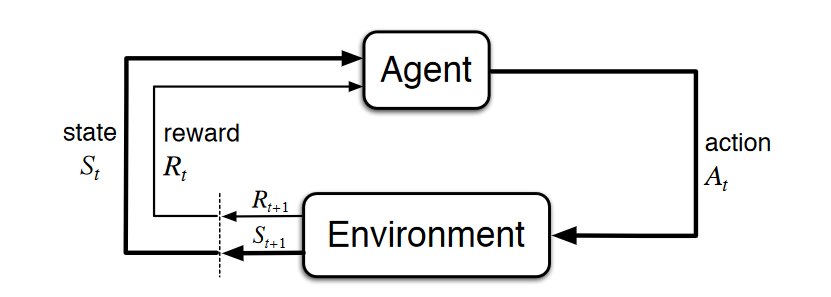
\includegraphics[width=0.75\linewidth]{figures/agent-environment.png}
	\caption{Agent-Environment Interface \cite{suttonReinforcementLearningIntroduction2014}}
	\label{fig:agent_environment}
\end{figure}

This interaction between agent and environment in Reinforcement Learning is modeled as a Markov Decision Process (MDP). This mathematical framework formalizes the decision process that satisfies the condition whereby future states depend only on the current state and action taken.

The agent-environment interaction is as shown in \autoref{fig:agent_environment} and depicts the agents taking actions $A_t$ in the environment and receiving reward $R_{t+1}$ and transitioning to the next state $S_{t+1}$ with probability $P$ at every discrete time step $k$. It is these cumulative rewards that the agent seeks to maximize over a specific time horizon. Furthermore the MDP problem can be characterized as a tuple of states, actions, rewards and a state transition function (model). Such that:

\begin{itemize}
	\item states: ($s\in S$) where $S$ is the finite state space.
	\item Actions ($a \in A$) where $A$ is the finite action space
	\item Transition probability: $f:X\times U \rightarrow X$ where $P(s_{t+1},r | s_t, a_t)$ is the state transition function
	\item Rewards: $r:S\times A \rightarrow \mathbb{R}$ where $r(s,a) = \mathbb{E}[R_t | S_{t-1} =s, A_{t-1} = a]$  is the reward function.
\end{itemize}


Furthermore, the agent follows a deterministic policy $\pi$ that establishes a mapping from states to actions, $\pi: S \rightarrow A$. The optimal policy seeks to maximize the total expected return (cumulative reward) of the agent where the return, $G_t$, is defined as some specific function of the reward sequence \cite{suttonReinforcementLearningIntroduction2014} as shown in \autoref{return_function}. 
\begin{equation}
	\begin{aligned}
		G_t  = R_{t+1} + R_{t+2} + R_{t+3} + \dots + R_{T} = \sum_{k=0}^TR_{t+k+1}
	\end{aligned}
	\label{return_function}
\end{equation}
However this is only relevant for scenarios where there is a time horizon and/or an idea of a final time step $T$ such as a task with some defined end point or events that are episodic in nature. This does not however extend to the greenhouse control problem and it does not necessarily follow a naturally identifiable episodes, and therefore the notion of an infinite time horizon with discounted returns is introduced. Where the return function now becomes:

\begin{equation}
	\begin{aligned}
		G_t  = R_{t+1} + \gamma R_{t+2} + \gamma^2 R_{t+3} + \dots = \sum_{k=0}^\infty \gamma^k R_{t+k+1} = R_{t+1} + \gamma G_{t+1}
	\end{aligned}
	\label{infinity_return}
\end{equation}

and the discount factor $\gamma \in [0,1]$. Although the return (\autoref{infinity_return}) is a sum of an infinite number of terms, it is still finite if the reward is nonzero and constant if $\gamma < 1$ \cite{suttonReinforcementLearningIntroduction2014}.As the discount factor, $\gamma$, approaches one, the the more future rewards are considered.  In contrast, values approaching zero render the agent "myopic," focusing solely on maximizing immediate rewards. The discount factor, $\gamma$, commonly fall within the range of 0.9 to 0.995 \cite{vandenbemdRobustDeepReinforcement}. This is an important concept since it can be shown that if the rewards are bounded (i.e. $\in R$) and a discount value of $\gamma <1$ is used, then a stable optimal policy can be found \cite{bertsekasNewtonMethodReinforcement2022}. There follows that a value function exists, under a specific policy $\pi$ of a state $s$, denoted as $v_{\pi}$ as the expected return starting in state $s$ and following the policy $\pi$ thereafter. This value function is depicted below in \autoref{value_function}.

\begin{equation}
	\begin{aligned}
		V_{\pi}(s) =  \mathbb{E}_{\pi}\left[{G_t | S_t = s}\right] =  \mathbb{E}_{\pi} 
		\left [\sum_{k=0}^{\infty} \gamma^k R_{t+k+1} | S_t = s \right], \forall s \in S 
	\end{aligned}
	\label{value_function}
\end{equation}

Given the absence of transition dynamics in a standard reinforcement learning (RL) problem, this can be extended for a state-action pair value function as in \autoref{eq:state-value_function} whereby $q_{\pi}$ denotes the expected return starting from state $s$ and taking action $a$, under the policy $\pi$ \cite{ajagekarDeepReinforcementLearning2022}.
\begin{equation}
	\begin{aligned}
		Q_{\pi}(s,a) =  \mathbb{E}_{\pi}\left[{G_t | S_t = s, At = a}\right] =  \mathbb{E}_{\pi}\left[\sum_{k=0}^{\infty} \gamma^k R_{t+k+1} | S_t = s, At = a\right]
	\end{aligned}
	\label{eq:state-value_function}
\end{equation}

Important to note, that from \autoref{infinity_return} and \autoref{value_function}, a value function under a generic stationary policy $\pi$ satisfies the Bellman equation as shown in \autoref{eq:bellman equation for value iteration} \cite{bertsekasNewtonMethodReinforcement2022,bellmanDynamicProgramming1966}.


\begin{equation}
	\begin{aligned}
		V_{\pi}(s) = \mathbb{E} \left[r(s,a) + \gamma V_{\pi}(s') \right] = \mathbb{E} \left[r(s,\pi(s)) + \gamma V_{\pi}(f(x,\pi(s))) \right]
	\end{aligned}
	\label{eq:bellman equation for value iteration}
\end{equation}

Moreover, the value function under the optimal policy, $\pi^*$ can be represented as shown in \autoref{Optimal bellman equation} and for the state-action value function in \autoref{Optimal state-action bellman equation}, where the relation between the value function and state-action value function is shown in \autoref{value and state-action relation} and \autoref{eq:q-function relation to value function}.

\begin{equation}
	\begin{aligned}
		V^*(s) =\max_{a} \mathbb{E} \left[r(s,a) + \gamma V^*(f(x,a)) \right]
	\end{aligned}
	\label{Optimal bellman equation}
\end{equation}

\begin{equation}
	\begin{aligned}
		Q^*(s,a) =\mathbb{E} \left[r(s,a) + \gamma \max_{a'}Q^*(s',a') \right]
	\end{aligned}
	\label{Optimal state-action bellman equation}
\end{equation}

\begin{equation}
	\begin{aligned}
		V^*(s) = \max_{a\in A} Q^*(s, a)
	\end{aligned}
	\label{value and state-action relation}
\end{equation}

\begin{equation}
	\begin{aligned}
		Q^*(s,a) = r(s,a) + \gamma V^*(s') 
	\end{aligned}
	\label{eq:q-function relation to value function}
\end{equation}

Finally, if the optimal state-action value function  (also known as Q-value) is known, then the optimal policy, $\pi^*$ can be found by \autoref{optimal policy} \cite{raoOPTIMALPOLICYOPTIMAL}, whereby the optimal policy greedily selects an action that maximizes the Q-value function.
Various methods exist to approximate this Q-value function, and it is this goal that reinforcement seeks to achieve. However it also possible to directly optimize the policy, $\pi$ to find the optimal policy $\pi^*$.

\begin{equation}
	\begin{aligned}
		\pi^*(s) = \arg \max_{a \in A} Q^*(s, a), \forall s \in S
	\end{aligned}
	\label{optimal policy}
\end{equation}

\subsection{Q learning}
These family of algorithms learn an approximating to the Q value function (\autoref{Optimal state-action bellman equation}). Moreover, these algorithms are ``off-policy'' algorithms whereby each update can use data collected at any point during training. Q learning offers a deterministic policy, whereby in each state, the action is selected based on \autoref{optimal policy}. In order to find the optimal Q value function, the update rule in \autoref{eq:q-learning update} is used in combination with a Q-table (a table that holds all possible combinations of states and actions). This iterative update rule aims to approximate the bellman equation in \autoref{Optimal state-action bellman equation}. Once the Q-function converges to the optimal Q-function, the optimal policy can be determined \cite{daveUnderstandingBellmanOptimality2021}.

\begin{equation}
	\begin{aligned}
		Q^{new}(s,a) = (1 -\alpha) \underbrace{Q(s,a)}_{\text{old value}} + \alpha \overbrace{(R_{t+1} + \gamma \max_{a'}(Q(s',a'))}^{\text{Learned value}}
	\end{aligned}
	\label{eq:q-learning update}
\end{equation}

where the temporal difference error is

\begin{equation}
	\begin{aligned}
		TD_{error} = (R_{t+1} + \gamma \max_{a'}(Q(s',a')) - Q(s,a)
	\end{aligned}
	\label{eq:temporal difference}
\end{equation}

Where TD error equals zero when optimality has been achieved (\autoref{Optimal state-action bellman equation}). However, this is only feasible for small problems, where the state and action space are small and discrete. In order to accommodate a continuous state space, the Deep-Q Network (DQN) was developed. In this approach, a neural network is utilized to estimate the Q-function, enabling the learning of a deterministic policy from data with high-dimensional features \cite{mnihPlayingAtariDeep2013}. However, DQN still outputs a discrete policy and therefore does not accommodate a continuous action space \cite{mnihPlayingAtariDeep2013}. Nevertheless, recent advancements have extended DQN's applicability to continuous action spaces.

\subsection{Policy Optimization}
Policy optimization offers a more direct approach in learning the optimal policy as apposed to Q-learning. Such algorithms represent a policy as $\pi_{\theta}(a|s)$, whereby $\pi_{\theta}(a|s)$ is a stochastic policy that gives the probabilities of choosing action $a$ given state $s$. The vector $\theta$ parameterize the policy, and it is these parameters that are optimized, by gradient ascent on the performance objective $J(\pi_{\theta})$ such as an \autoref{eq:policy_update}.


\begin{equation}
	\begin{aligned}
		\theta_{t+1} = \theta_{t} + \alpha \hat{\nabla J(\theta_t)}
	\end{aligned}
	\label{eq:policy_update}
\end{equation}

Here, $\hat{\nabla J(\theta_t)}$ represents a stochastic estimate, where its expected value approximates the gradient of the performance objective function with respect to the policy's parameters, $\theta$ \cite{suttonReinforcementLearningIntroduction2014}. Such algorithms are called ``on-policy" algorithms, which mean that each update is performed from data that was collected from the most recent version of the policy.
All RL algorithms that follow this update rule on the policy are considered policy gradient/optimization methods, whether or not they also learn an approximation to a value function. However, such algorithms are often called actor-critic methods \cite{suttonReinforcementLearningIntroduction2014}.  Policy Optimization algorithms are also naturally able to handle continuous state and action spaces.


\subsection{Actor-Critic}
Perhaps a more interesting class of RL algorithms combines both q-learning and policy optimization. Policy optimization methods directly optimize the policy, therefore they tend to be more stable and reliable in contrast to Q-learning and are better for continuous and stochastic environments \cite{suttonReinforcementLearningIntroduction2014}. However, because Q-learning learns ``off-policy'', it has a substantially higher sample efficiency than that of policy optimizations methods \cite{suttonReinforcementLearningIntroduction2014}.
Actor-critic methods often incorporate the strengths from both policy gradient methods and q-learning, in order to achieve stable and fast learning. The critic learns a value function and the actor learns a policy. The critic provides feedback on how good an action was and uses this to update the policy. In this way, the actor can learn from both its own experience and the critic's feedback 
Moreover, actor-critic algorithms are also suitable in tackling continuous state and action spaces \cite{suttonReinforcementLearningIntroduction2014}.

\subsection{SAC}
\emph{A brief explanation of how SAC works and how it learns}


\section{MPC}
\subsection{Why MPC for Greenhouse Control?}
Among others, MPC excels at handling constrained Multiple Input, Multiple Output (MIMO) systems, rendering it highly effective in such situations, such as greenhouse control. Moreover, MPC's ability to handle non-linear dynamics and its optimality has contributed to its widespread adoption and has become the standard approach for implementing constrained multivariable control in the process industry \cite{daiDiscreteTimeModelPredictive2012}. Nearly every application introduces constraints, whether it be on the state of the system or the control inputs. Actuators,constrained by physical and safety limits such as temperature or pressure control, makes it necessary for controllers to handle such constraints. While the online computational time for such controllers may be expensive, for slow dynamics such as a greenhouse, sufficient computational time is available to accommodate this. Furthermore, the ongoing trend of faster computation mitigates this concern, making it less of a problem.
Although many control schemes exist in controlling greenhouses, it has been shown that an MPC controller outperforms an adaptive PID controller for greenhouse air control in \cite{ghoumariNonlinearConstrainedMPC2005}. Even though the control of a greenhouse is inherently non-linear, non-linear Model Predictive Control (MPC) schemes have demonstrated effectiveness in handling this complexity, as evidenced in \cite{gruberNonlinearMPCBased2011, montoyaHybridcontrolledApproachMaintaining2016} specifically for temperature control in a greenhouse. Furthermore, \cite{bersaniModelPredictiveControl2020} shows insight of the performance of MPC when optimized for energy savings of a greenhouse, displaying impressive results over set-point tracking controllers. Further, \cite{boersmaRobustSamplebasedModel2022} successfully implements a robust MPC to control the economic benefit of a greenhouse with parametric uncertainty, displaying its potential in greenhouse control. Moreover, as confirmed by \cite{bersaniModelPredictiveControl2020}, MPC stands out as the most effective control approach in smart greenhouses for energy savings. The study concludes that MPC is particularly advantageous when the system's dynamics can be reasonable approximated by a model and are sufficiently slow relative to the required time needed to perform the optimization.

Additionally, MPC has been shown to have a strong theoretical foundation. Researches have developed rigorous methods in analysing performance and stability on a MPC under certain conditions, including the optimality and robustness of the implemented controller. Indeed, if the system dynamics are known, it is possible to design an MPC to fulfill specific design requirements. \cite{rawlingsModelPredictiveControl2017}

\subsection {The General MPC problem}
Model Predictive control (MPC) is a control strategy whereby the current control input is computed by solving on-line, a finite horizon open-loop optimal using the systems current state.
The MPC controller is an intuitive controller, whereby MPC aims to solve the infinite-horizon optimal control problem (OCP) as a series of finite-horizon problems in order to make the problem computationally tractable \cite{beckenbachAddressingInfinitehorizonOptimization2018}. The formulation of the MPC optimization problem involves finding a sequence of control actions that minimizes a cost function $J$ subject to constraints over a specific time horizon. The first step of the control strategy applied to the system, and at the subsequent time step, the system is sampled again and the entire process is recalculated providing an updated control plan. This cost function is tailored to the specifics of the MPC application \cite{rawlingsModelPredictiveControl2017}. While this approach is not optimal, it is an approximation of the infinite time horizon problem and has been shown to yield excellent results in practice as discussed above. The choice of prediction horizon length is often a trade-off between computational efficiency and the desired control performance. 

While MPC can be used for both continuous and discrete time system dynamics, however continuous system must be discretized to render the Optimal Control Problem (OCP) tractable. This is necessary since a continuous time system gives rise to an infinite-dimensional problem. Therefore the discrete case will be considered as illustrated:

\begin{equation}
	\begin{aligned}
		& \hat x(k+1) = f(\hat x(k),u(k),w(k),e(k), \hat p) \\
		& y(k) = g(\hat x(k),u(k),w(k),e(k))
	\end{aligned}
	\label{eq: discrete system dynamics}
\end{equation}

where:
\begin{itemize}
	\item $f(\cdot)$ is the system dynamics
	\item $y(k)$ is the output of the system
	\item $\hat x(k) \in \mathbb X,$ is the estimated state of the system 
	\item $u(k) \in \mathbb U,$ is the input of the system
	\item $w(k)$ is the measurable disturbances 
	\item $e(k)$ is the unmeasurable disturbances 
	\item $\hat p$ is the uncertain parameters of the model
\end{itemize}

It is possible that the state may be unknown, and therefore a state estimation is required, however we will further assume that the state is fully measurable or perfectly estimated, i.e. $\hat x(k) = x(k)$.
When considering a finite-time horizon, $N_p$, The OCP problem can be formulated as in \autoref{eq:mcp ocp}.

\begin{equation}
	\begin{aligned}
		& \min_{x(k_0:N_p+1),u(k_0:N_p)} J(x(k),u(k)) = \\ 
		& \min_{x(k_0:N_p+1),u(k_0:N_p)} \sum_{k=k_0}^{N_p} l(x(k),u(k)) + G_T(x(N_p +1))  \\
		\text{s.t.} \quad  & x(k_0) = x_{k_0}                              & \forall k = k_0,\hdots, N_p,\\
		& x(k+1) = f(x(k),u(k),w(k),e(k), \hat p)       & \forall k = k_0,\hdots, N_p,\\
		& y(k) = g(x(k),u(k),w(k),e(k))                 & \forall k = k_0,\hdots, N_p,\\
		& g(x(k),u(k),w(k)) \leq 0                      & \forall k = k_0,\hdots, N_p,\\
		& x_{lb} \leq x(k) \leq x_{ub}                  & \forall k = k_0,\hdots, N_p,\\
		& u_{lb} \leq u(k) \leq u_{ub}                  & \forall k = k_0,\hdots, N_p,\\
		& |u(k) - u(k-1)| \leq \delta                   & \forall k = k_0,\hdots, N_p,\\
	\end{aligned}
	\label{eq:mcp ocp}
\end{equation}

where $x(k_0:N_P+1)$ denotes a sequence of states, i.e. $[x(k_0), x(k_0+1), \hdots, x(N_P+1)]^T$ and may be denoted as $\bold{x}$ and similarly for the control actions $\bold{u}$ and known disturbances $\bold{w}$. The cost function $J(\cdot)$ may be explained by a stage cost $l(\cdot)$, where $l: \mathbb X \times \mathbb U \rightarrow \mathbb R$, which is the cost incurred at every time step $k$ based on the current state and input applied and a terminal cost, $G_T(\cdot)$, which accounts for the cost associated with the state at the end of the prediction horizon. \cite{daiDiscreteTimeModelPredictive2012,boersmaRobustSamplebasedModel2022}. The inequality constraints may be collected in a vector $\bold{G(\bold{x,u,w})}$ where $\bold{G} < 0$ and the equality constraints (system dynamics) in $\bold{H(\bold{x,u,w})}$ where $\bold{H(\bold{x,u,w})}=0$ over the prediction horizon.\\

It is noted that the more accurate the model, the better the prediction and thus the better the actions. In the case of greenhouse control, if the model accurately captured all crop and greenhouse phenomena, state constraints would not be needed, since these constraints would be naturally incorporated into the dynamics. However, in practice, such dynamics are often still captured by explicit constraints. Moreover, an increasing complexity in the prediction model often leads to an increase in computational time and power which may exceed the time-scale of the system. This can make control actions impractical or infeasible within the required time frame \cite{rawlingsModelPredictiveControl2017}. Greenhouse environments are known to be complex and highly non-linear in nature. Hence, for control purposes,  it is necessary to have simplified models that accurately predict system dynamics such as the model presented by van Henten \cite{hentenGreenhouseClimateManagement1994} and as discussed in \autoref{greenhouse_model} for greenhouse control. 

Moreover, uncertainties in the model may greatly impact the performance of the MPC and the relation between a deterministic model and an uncertain model is explored in \cite{boersmaRobustSamplebasedModel2022} and shown that even when a robust MPC strategy is used a $20\%$ in relative parametric uncertainty decreased the crop yield by $11\%$.

\subsection{EMPC}
The goal of most current advanced control systems is to guide a process to a target set point rapidly and reliably. The steady state is often determined by a different layer of control, known as the real-time optimization (RTO) layer. This layer ensures that the current steady-state brings the greatest economic benefit. Subsequently, MPC is employed to steer the process towards this optimized steady state. However, this separation in control information is not necessarily desirable and/or optimal in regards to maximizing economic benefit. This economic benefit could refer to the profitability, efficiency and/or sustainability of the controlled process \cite{ellisTutorialReviewEconomic2014}. Thus, Economic Model Predictive Control (EMPC) is introduced, wherein the economic objective is directly incorporated as the objective function of the optimal control problem that the MPC aims to minimize \cite{rawlingsFundamentalsEconomicModel2012}. Here, $l(x,u)$ is replaced by $l_e(x,u)$ in \autoref{eq:mcp ocp}, 
that encapsulates an economic model of the process.

By adopting this approach, it becomes feasible that dynamic, transient or time varying operation of the process could lead to higher economic benefit as compared to controlling the process to an optimal steady-state. As stated in \cite{rawlingsFundamentalsEconomicModel2012}, incorporating the the economic model directly into the cost function does not assume the structure of the stage costs as presented in \autoref{eq: assumption on stage cost for standard mpc} and therefore has no stability guarantees. 
Furthermore, the closed-loop performance of the EMPC does not consider the system's dynamics, and although it optimizes the process economics, it does so over a finite time horizon. Therefore, over a long period of operation, there is in general no closed-loop performance guarantees under EMPC \cite{ellisTutorialReviewEconomic2014}.
\cite{rawlingsFundamentalsEconomicModel2012} further showed  in the case of a chemical plant, despite the increase in economic benefits, the controller resulted in unstable plant dynamics which is highly undesirable for such a process. In order to achieve stability, a terminal constraint in the optimal control problem is introduced \cite{amritEconomicOptimizationUsing2011}. This terminal constraint must be selected carefully to achieve stability \cite{rawlingsFundamentalsEconomicModel2012}. However, \cite{amritEconomicOptimizationUsing2011}, introduces a terminal cost function and demonstrates its superiority over a terminal constraint in terms of performance while maintaining system stability. Although, it is possible to fabricate a terminal cost/constrain to achieve desired closed-loop performance and stability, authors of \cite{rawlingsFundamentalsEconomicModel2012}, \cite{amritEconomicOptimizationUsing2011} and \cite{ellisTutorialReviewEconomic2014} acknowledge the difficulties in constructing such an appropriate terminal cost/constrain. Limited works provide theoretical analysis in order to construct an appropriate terminal cost in the absence of stability constraints. Most often, simulations are performed to design cost functions suitable for the specific application. Importantly, only two methodologies exist to assure closed-loop performance: to use a sufficiently large horizon or the application of an appropriate terminal constraint \cite{ellisTutorialReviewEconomic2014}. As will be discussed later, stability of the system's dynamics is not a concern, due to the nature of the desired controlled system in this thesis.

\section{RL and MPC in tandem}
Reinforcement Learning (RL) and Model Predictive Control (MPC) are both techniques used in the field of control theory, but they have distinct approaches and strategies. While RL and MPC share the overarching goal through optimal control, their methodologies differ, with RL focusing on learning from interactions and MPC relying on model-based optimization over a finite time horizon. 
Both control algorithms bring their respective advantages and disadvantages, with extensive similarities between the two. It becomes evident to merge the two strategies in the hope of creating a control scheme that combines the benefits of both. 

MPC finds optimality in solving a finite-horizon problem in a receding fashion.  In this process, the controller is recognized for its sample efficiency, robustness and constraint handling. However, it falls short in terms of adaptability. Moreover, large and complex systems may lead to a non-convex optimization problem which are computationally expensive to solve and may lead to sub-optimal control. Finally, model mismatch and uncertainties in forecasted disturbances can lead to a significant deterioration in control effectiveness \cite{arroyoReinforcedModelPredictive2022}.

While reinforcement learning (RL) is predominantly explored within the machine learning community, its usefulness in the control space is undeniable. Its ability to learn from interactions with the environment leads to its high adaptability and uncertainty handling, however it struggles with constraints. The quality of control is strongly influenced by the training of the reinforcement learning (RL) algorithm. Nevertheless, the popularity of RL in control research persists due to its capacity to handle complex systems. Although RL might suffer from the curse of dimensionality, necessitating a reduction of states and control action, the introduction of neural networks and actor-critic algorithms addresses this issue.


Several methods are available that seek to integrate the two control schemes, shedding light on the strengths and weaknesses of the resulting controller with respect to its specific application. There are two main ways to combine RL and MPC, either by truncating the objective function of the MPC (or rolling out the bellman-equation) or using the MPC as the function approximator of the learning agent. The former strategy will be further explored in this thesis.

To differentiate this thesis from the concept of employing Model Predictive Control (MPC) as a function approximator, a concise explanation will be provided. This aims to clarify to the reader what the thesis does not focus on. As discussed in \autoref{sec:rl}, the DQN is usually implemented as a neural network and is parameterized by a vector $\bold{\theta}$. The approximated value of a state $s$, parameterized by a weight vector  $\theta$ is then given as $ \hat{v}(s,\theta) = v^*(s)$ where $\hat{v}$ \cite{lubbersAutonomousGreenhouseClimate2023}. However, it is possible to use a MPC scheme instead of a neural network to facilitate parametrization for approximating the value function and policy. This is the goal of using MPC as a function approximator for RL. This thesis does not explore this concept. It instead explores the design and implementation of an (E)NMPC algorithm that utilizes the value function learned by RL in its optimal control problem formulation to propagate information beyond the prediction horizon. 

In order to gain insight in how the two optimal schemes will be combined, it is imperative to understand the differences and similarities of the two algorithms. Key areas such as the approach, optimality, computational effort and prediction horizon will be discussed and compared in order to motivate and understand the connection between the two control schemes. This section summarizes \cite{arroyoReinforcedModelPredictive2022} works with added literature from \cite{bertsekasNewtonMethodReinforcement2022} and \cite{linReinforcementLearningBasedModel2023}.

\subsection{The Optimality}
 As mentioned in \autoref{sec:rl} and \autoref{sec:mpc}, both control strategies are optimal in that they attempt to solve the infinite prediction horizon problem.

The quality of the solution obtained through MPC is subject to the accuracy of the prediction model, which is further simplified to reduce computational burden. However, optimality of the direct optimization methods of the MPC problem is obtained through the Karush–Kuhn–Tucker conditions which are necessary conditions for optimality. Moreover, the local optimal policy obtained may also be sub-optimal due to multiple local optima in the case of non-linear optimization problems.

In contrast, if the state space is countable and the MDP is perfectly known, DP algorithms (which relay on Bellman's principle), offer sufficient conditions for global optimality. However, these algorithms are significantly impacted by the curse of dimensionality. Consequently , approximations are used such as RL. 
Although RL can only guarantee optimality under specific conditions when solving the Bellman equation \autoref{eq:optimal bellman equation}, the approximated value function contains global optimal information so that the infinite-horizon control policy may be obtained \cite{linReinforcementLearningBasedModel2023}. It is important to note that this is only an approximation. Moreover, RL does not directly impose state and control constraints. While it is possible to indirectly incorporate these constraints through the reward function, such an approach does not ensure that the optimal policy obtained will inherently adhere to these constraints. This becomes an issue when the problem at hand is safety critical.
\subsection{Computational Effort}
 The online computational cost of MPC stands out as one of the principal drawbacks of this control strategy, particularly when dealing with complex models featuring numerous variables to optimize. Thus the model is often simplified, resulting in sub-optimal policies. In comparison to DP and RL algorithms, large computational power is expended training the policy, even for simple systems. However, once training is completed, the estimated optimal action may be given by a function evaluation of the policy. The evaluation of the policy, typical through a feed forward pass of a neural network, leads to a limitation in flexibility, especially in continuous control scenarios. Moreover, in obtaining an accurate value function proves to be difficult due to instability, rank loss and overestimation bias of the value function. This is especially prevalent for complex non-linear systems such as a greenhouse.
 
\subsection{The Prediction Horizon}
Arguably, the most crucial characteristic of both control strategies lies in their respective prediction horizon. Both are predictive controllers, with Model Predictive Control (MPC) employing explicit optimization over a finite prediction horizon to determine the optimal control action. On the other hand, Reinforcement Learning (RL) explores and interacts with its environment to learn the optimal action, optimizing for both immediate and discounted future rewards.
Hence, a shortcoming of MPC is the finite prediction horizon. This limitation becomes even more pronounced when dealing with sparse rewards and slow system dynamics. In such cases, actions taken at the current time step may only yield rewards past the prediction horizon, causing the MPC controller to be myopic. It is possible to counteract this drawback with an extended prediction horizon, however, as discussed, this increases the complexity and computational burden of the controller.

In contrast, RL aims to predict the optimal action to take over an infinite time horizon by incorporating a discount factor on rewards.This discount factor provides a measure of how much future rewards contribute to determining the optimal action. This bears similarities to the prediction horizon concept employed in MPC controllers. For RL, it can be shown, through geometric series convergence thatthe prediction horizon of the MPC controller is equivalent to $N_p = 1/(1 - \gamma)$ \cite{arroyoReinforcedModelPredictive2022}.
It is noted that the prediction horizon over the RL can extend to infinite when $\gamma = 1$, however convergence of the total rewards gained is not guaranteed,  emphasizing the significance of the discount factor $\gamma$. Nonetheless, discounted infinite prediction horizons generally result in improved long-term behaviour. However, as stated in \cite{arroyoReinforcedModelPredictive2022}, RL makes less efficient use of forecasted information. This inefficiency arises because all future knowledge is condensed and presented to the agent's observation without retaining its time dependency. Consequently, the agent is required to implicitly learn the system's dynamics through interactions with the environment, leading to the difficulty of understanding the time dependency of its actions on future rewards. In comparison, MPC naturally preserves the time dependency since it has the system’s dynamics formulated in its problem, however since it only looks N steps forward, it produces a locally optimal policy \cite{linReinforcementLearningBasedModel2023}. A synergistic approach to combining the two control strategies would be to have a MPC controller optimize a short prediction horizon while propagating global information provided by RL. This integration of the two controllers is further justified in the context of greenhouse dynamics, where actions executed at the current time step may result in rewards that manifest over the long term. Finally, as outlined in \autoref{sssec:empc} within the work of \cite{ellisTutorialReviewEconomic2014}, it is imperative, when employing an EMPC, to construct the optimal control problem with an adequate terminal constraint to ensure the performance of the system.  This terminal constraint, which must encapsulate information beyond the prediction horizon, underscores the evident synergy with the value function acquired through RL to provide the required information for the desired system performance.


